\section{Grundlegende Architektur}\label{sec:architecture}

\begin{figure}
	\centering
	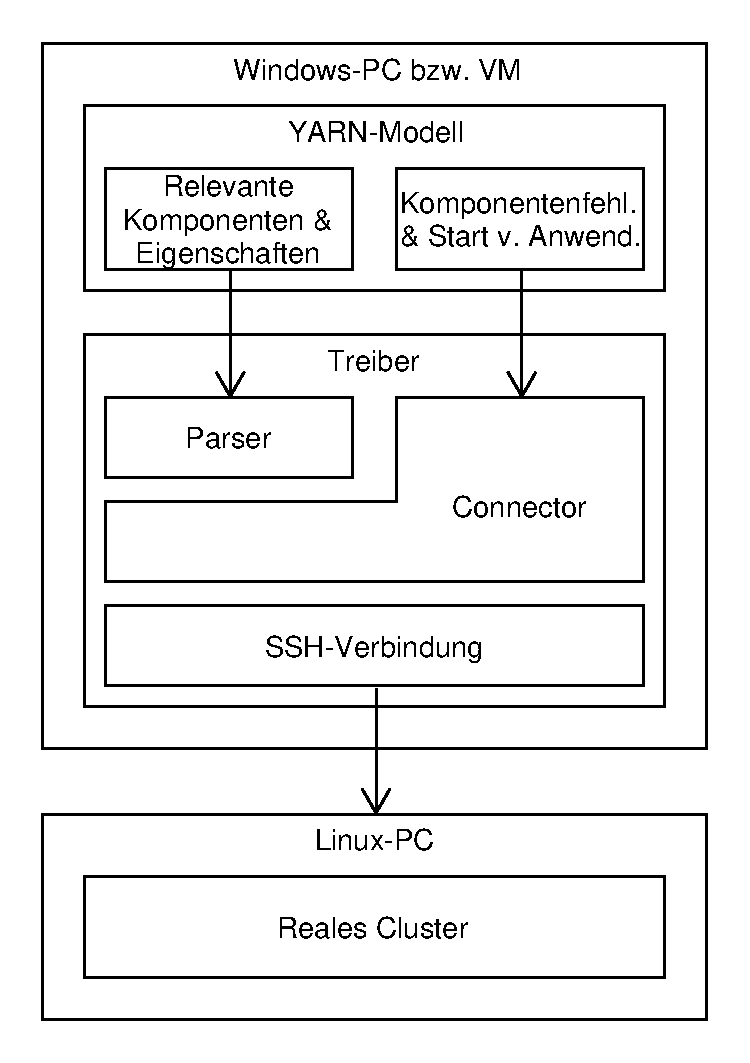
\includegraphics[width=.8\columnwidth]{./images/modelArchitecture.pdf}
	\caption{Grundlegende Architektur des Gesamtmodells}
	\label{fig:modelArchitecture}
\end{figure}

Die grundlegende Architektur des gesamten Aufbaus besteht aus drei Schichten, dem eigentlichen YARN-Modell, dem realen und zu testendem Cluster und dem SSH-Treiber, welcher das Modell mit dem realen Cluster verbindet (\autoref{fig:modelArchitecture}).